\begin{fullwidth}
    \section{A Front End Incentives Program} \label{sec:feip}

    \begin{adjustwidth}{2cm}{2cm}
        \justify
        With a larger focus on decentralization, new behaviors in the dYdX ecosystem might need to be incentivized, including the operation of front ends, and indexers. In this section, we describe a program to incentivize the deployment, maintenance, and decentralization of the dYdX Front End. We discuss why such a program might be necessary, and how it could be implemented with minimal surface area for value extraction from adversarial players. We further discuss how the community might leverage such a program to incentivize the deployment of Front Ends in strategic regions, with support for specific languages, or the addition of strategic features.
    \end{adjustwidth}
    
    \textcolor{gray}{\rule{\linewidth}{0.1mm}}
\end{fullwidth}

    dYdX Trading has been developing three front ends for non-programmatic users, including one for the web, one for iOS, and one for Android. The team has recently open-sourced the code for operating these front ends, such that anyone can deploy and host the front end themselves. See the corresponding GitHub repository \bhref{https://github.com/dydxprotocol/v4-web}{here}. We asked Joseph Axisa (also known as @ImmutableLawyer on the dYdX forums) to explain why decentralizing the front end is at the core of a truly decentralized protocol:

    \begin{displayquote}
        In a \bhref{https://immutablelawyer.substack.com/p/frontend-decentralisation}{post} on Substack (derived from a previous forum post of mine from the dYdX Forums) titled, ‘Frontend Decentralisation’ I discussed the importance of decentralising the frontend, the corresponding importance thereof and the factors that have to be taken into account so as to achieve a sufficient level of decentralisation at the frontend layer of a project. To put it simply, the frontend is the first point of access enabling users to interact with the underlying codebase. Thus this layer is an integral part of any project. 

        In most cases, this pivotal piece of infrastructure is controlled in a centralised manner by one entity or a group of entities that back (directly or indirectly) the development of the project. This, naturally, gives rise to an increase in the project’s centralisation, an increase in censorship risk and also introduces a single point of failure.
    \end{displayquote}

    \begin{marginfigure}
        \centering
        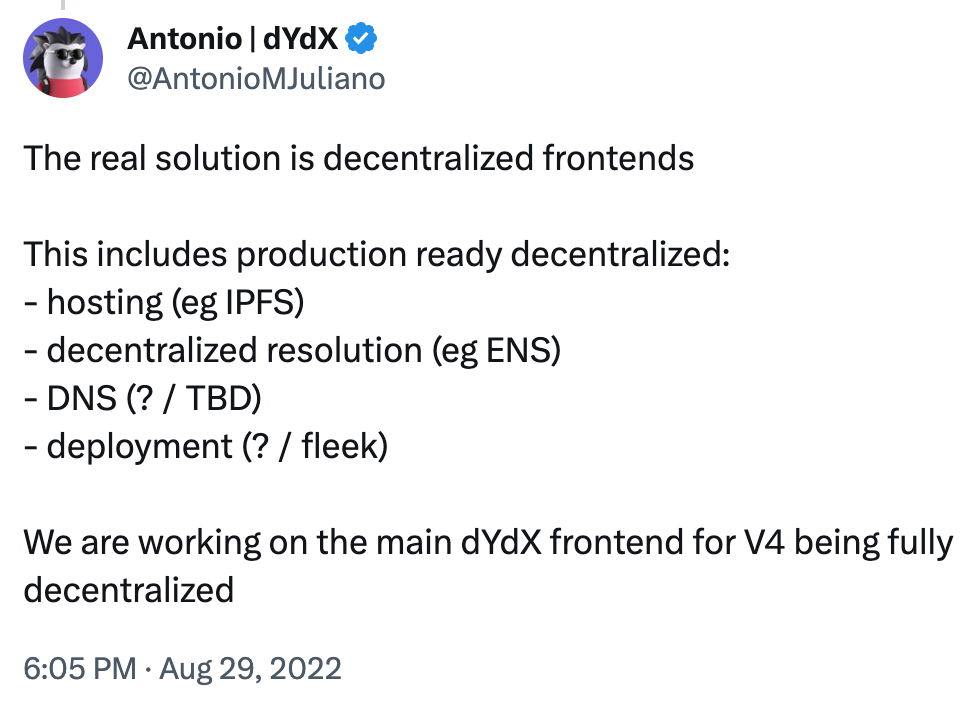
\includegraphics[width=\linewidth]{figs/feip_tweet.png}
        \captionsetup{width=\linewidth}
        \caption{\bhref{https://twitter.com/AntonioMJuliano/status/1564373755517751296?s=20}{Tweet} by Antonio Juliano, Founder and CEO of dYdX Trading, on decentralizing the front end.}
        \label{fig:feip_tweet}
    \end{marginfigure}

    That is, decentralizing the front end is about eliminating single-points-of-failure from the dYdX protocol and making it more robust to a number of censorship risks. Given the current uncertain regulatory environment in the United States and other major jurisdictions, it is increasingly important to decentralize such a sensitive component of the protocol's stack.

    \subsection{The Challenge of Decentralization}

        Decentralization, of course, does not come easily.

        By decentralizing the front end, dYdX will now require a cohort of ``front end operators'' to deploy and maintain the dYdX v4 front end. This requires some financial resources to pay the necessary software developers, service the necessary server costs, and pay for any additional developer tools required to keep the site or application running. As we will discuss, the dYdX Operations Trust was funded, in part, to support the deployment of the dYdX v4 front end. However, no additional funds have been committed to incentivize the deployment and maintenance of front ends from other teams and in other jurisdictions. This section is devoted to the possibility that an insufficient number of front ends are deployed and maintained following the launch of dYdX Chain. 
    
        \sidenotequote{The FTC reports that crypto scams have increased by an incredible 900 percent since the start of the Pandemic.}{\bhref{https://dfr.vermont.gov/consumer-alert/investor-alert-npr-report-crypto-fraud-illustrates-need-caution}{Department of Financial Regulation, State of Vermont}}Aside from the possible lack of financial incentives, we also consider the user risks of decentralizing the front end. Under a decentralized front ends paradigm, the dYdX community might expect an increase in fraudulent or risky activity from malicious front ends, such as applying hidden fees, performing unnecessary data collection, or tricking users into signing fraudulent transactions. 
    
        That is, decentralizing dYdX's front end expands the surface area of attack for malicious actors. Consider \bhref{https://www.volexity.com/blog/2022/12/01/buyer-beware-fake-cryptocurrency-applications-serving-as-front-for-applejeus-malware/}{this} novel attack performed by North Korea's Lazarus Group, where victims are directed to a clone of a well-known website and tricked into downloading malware targeting their private keys. It has been described in greater depth by the FBI and CISA \bhref{https://www.cisa.gov/news-events/cybersecurity-advisories/aa21-048a}{here}. 
    
        \begin{figure}[H]
            \centering
            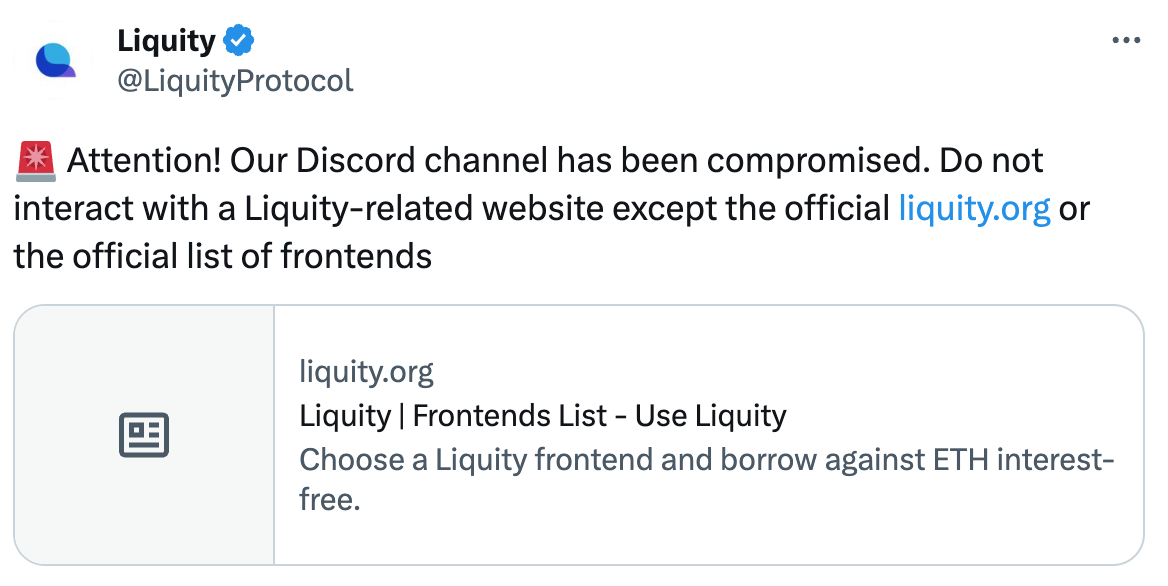
\includegraphics[width=0.5\linewidth]{figs/liquityscam.png}
            \captionsetup{width=0.5\linewidth}
            \caption{\bhref{https://twitter.com/LiquityProtocol/status/1627605124985024512}{Tweet} by @LiquityProtocol regarding a Discord scam targeting retail users with malicious front ends.}
            \label{fig:liquityscam}
        \end{figure}

    \subsection{Introducing a Front End Incentives Program}
    
    With this in mind, we consider a potential incentives program that governance can use to influence the dYdX front end experience. In doing so, governance can encourage benign front end operators that abide by certain community-owned standards, and simultaneously direct retail users to those front ends and away from the malicious ones. We purport the following objectives for a Front End Incentives Program.
    
    \begin{enumerate}
        \item \textbf{Decentralization:} Incentivize the deployment of multiple separate front ends.
        \item \textbf{Protection:} Foster a community-owned process for signaling ``safe'' front ends to retail users.
        \item \textbf{Curation:} Incentivize front ends to abide by certain community-owned standards, and potentially incentivize new experiences.
    \end{enumerate}
    
    Addressing objective 2 (protection) does not rely on any financial incentives, and we may establish and streamline governance processes to address it soon after the Genesis of dYdX Chain. This whitelisting process, as we will discuss, would be a community-owned version of the Liquity front ends list, shown in Fig. \ref{fig:liquityscam}.\sidenotequote{The responsibilities of a deployer will include:
            \begin{itemize}
                \item Acquiring and owning web domain
                \item Meeting deployment prerequisites:
                Installing Node.js 16 and npm locally
                Setting up web3.storage account
                Setting up Cloudflare account 
                \item Initial deployment of frontend
                Download of front end codebase and deployment script from dYdX Github
                Running deployment script to pin the files to IPFS and update the IPFS hash
                \item Updating frontend
                Following the dYdX Github repos to get codebase updates
                Running the deployment script when new codebase updates are available to pin the updated files to IPFS and update the IPFS hash
                \item Setup of ancillary accounts
            \end{itemize}
            }{\bhref{https://dydx.exchange/blog/v4-deep-dive-front-end}{v4 Deep Dive: Front End}
        }
    
    Objectives 1 and 3 rely on financial incentives from the community treasury, and as such may be deployed if and when governance deems it necessary. It may be appropriate to launch such an incentives program if we observe an insufficient amount of front ends being deployed, or if existing front ends are not providing an adequate experience for retail users - such as not providing appropriate risk disclaimers, or charging excessive additional fees.

    \subsection{Whitelisting: A dYdX Front End Registry}

        A key component of decentralizing the front end is mitigating the damage caused by scams and attacks on retail traders. As we see in Fig. \ref{fig:liquityscam}, Liquity has an official website that links to a selection of Liquity front ends. Here, we propose how governance may host a similar registry of high-quality front ends that signals to users which front ends are safe, and whether they abide by certain minimum community-owned standards, discussed in the following Section.
        
        We consider a whitelisting process that resembles Lido's \bhref{https://easytrack.lido.fi/}{EasyTrack} program. Front end operators may submit proposals to be added to the front end registry, which will pass by default. Voters may then veto the submission if an applicant or application is found to be suspicious. By setting the default outcome of the proposal to be a success instead of a failure, we minimize governance overhead and expedite the process for onboarding new front ends. This might be further expedited by creating a subDAO to oversee dYdX's front ends, or adding this as a responsibility to an existing subDAO.
        
        Existing dYdX subDAOs may maintain a separate website that hosts the registry, and the registry may be duplicated in a pinned forum post. We provide an example for a submission to add a new front end to the dYdX front end registry:

        \callout{[DRC] Add ABC.com to the Front Ends Registry}{ 

        ABC.com is a front end hosted by ABC LLC in Lebanon and written in Arabic. 
        
        \vspace{0.25cm}
        
        \begin{itemize}
            \item <Company description>
            \item <Product Description>
            \item <Contact Information>
            \item <Product Screenshots>
        \end{itemize}   
        
        \vspace{0.25cm}

        \begin{center}
            \textbf{Voting}
        \end{center}
        
        \begin{itemize}
            \item \textbf{Veto.} Veto this proposal.
        \end{itemize}}

        Applications could be reviewed by governance or a dedicated subDAO. Applicants might be individual contributors, or larger aggregators such as DeFi Saver or Instadapp\sidenote{DeFi Saver and Instadapp are two of the largest front end providers for \bhref{https://www.liquity.org/frontend}{Liquity}.}. 

        This whitelisting process also underpins the front end incentives program proposed in this report. Without a whitelisting process, adversarial users might be able to ``farm'' the incentives program. Furthermore, a lack of a whitelisting process would constrain the design of the incentive formula, precluding formulas that flatten the distribution of incentives, due to a problem known as ``Sybil Resistance''.

    \subsection{Community Standards}

        dYdX Trading has curated a successful user experience for v3 traders and we can expect that the front end for v4 will similarly provide a great experience for traders using a direct fork of their open source code. However, decentralizing the front end means front end operators can change, improve, or worsen the front end experience for their users. Over time, the dYdX community may choose to curate a set of minimum community standards for adequate front ends. These may include:

        \begin{itemize}
            \item Not charging excessive additional fees from users.
            \item Not collecting unnecessary browser data from users.
            \item Appropriate disclaimers for permissionless markets, markets with excessive price volatility, or markets with excessive external rewards. These disclaimers are similar to the disclaimers on Osmosis Zone, depicted in Fig. \ref{fig:frontierwarning}.
        \end{itemize}

        Using the whitelisting process discussed above, and the incentives program we will design in the following sections, governance may wield a small portion of the community treasury to encourage front end operators to abide by these standards and protect the retail experience.

    \subsection{Incentive Alignment and Opportunity Sizing}

        \nonumsidenote{The dYdX Operations Trust (DOT), has received funding to deploy and maintain the three front ends, as well as hire a 3rd party contractor to operate the v4 indexer. Read more about it in \bhref{https://dydx.forum/t/dydx-operations-subdao-v2/274}{this forum discussion}.}We now present an incentives program designed to incentivize front end operators proportionally to the value they contribute to the dYdX ecosystem.
        
        Consider an incentives program that offers front end operators a share of the fees generated by users trading on their platform. This creates sustainable value alignment between the front end operators and the protocol: operators are incentivized to increase trading fees by acquiring more users and increasing trading volume. Front end operators might:

        \begin{itemize}
            \item Integrate dYdX v4 with existing DEX aggregators, mobile apps, or payment services.
            \item Develop front ends in various different regions and languages, increasing accessibility and awareness, and reducing regulatory exposure to particular countries or blocs.
            \item Develop new and innovative features to complement the existing front end product.
        \end{itemize}

        \begin{figure}[htp]
            \centering
            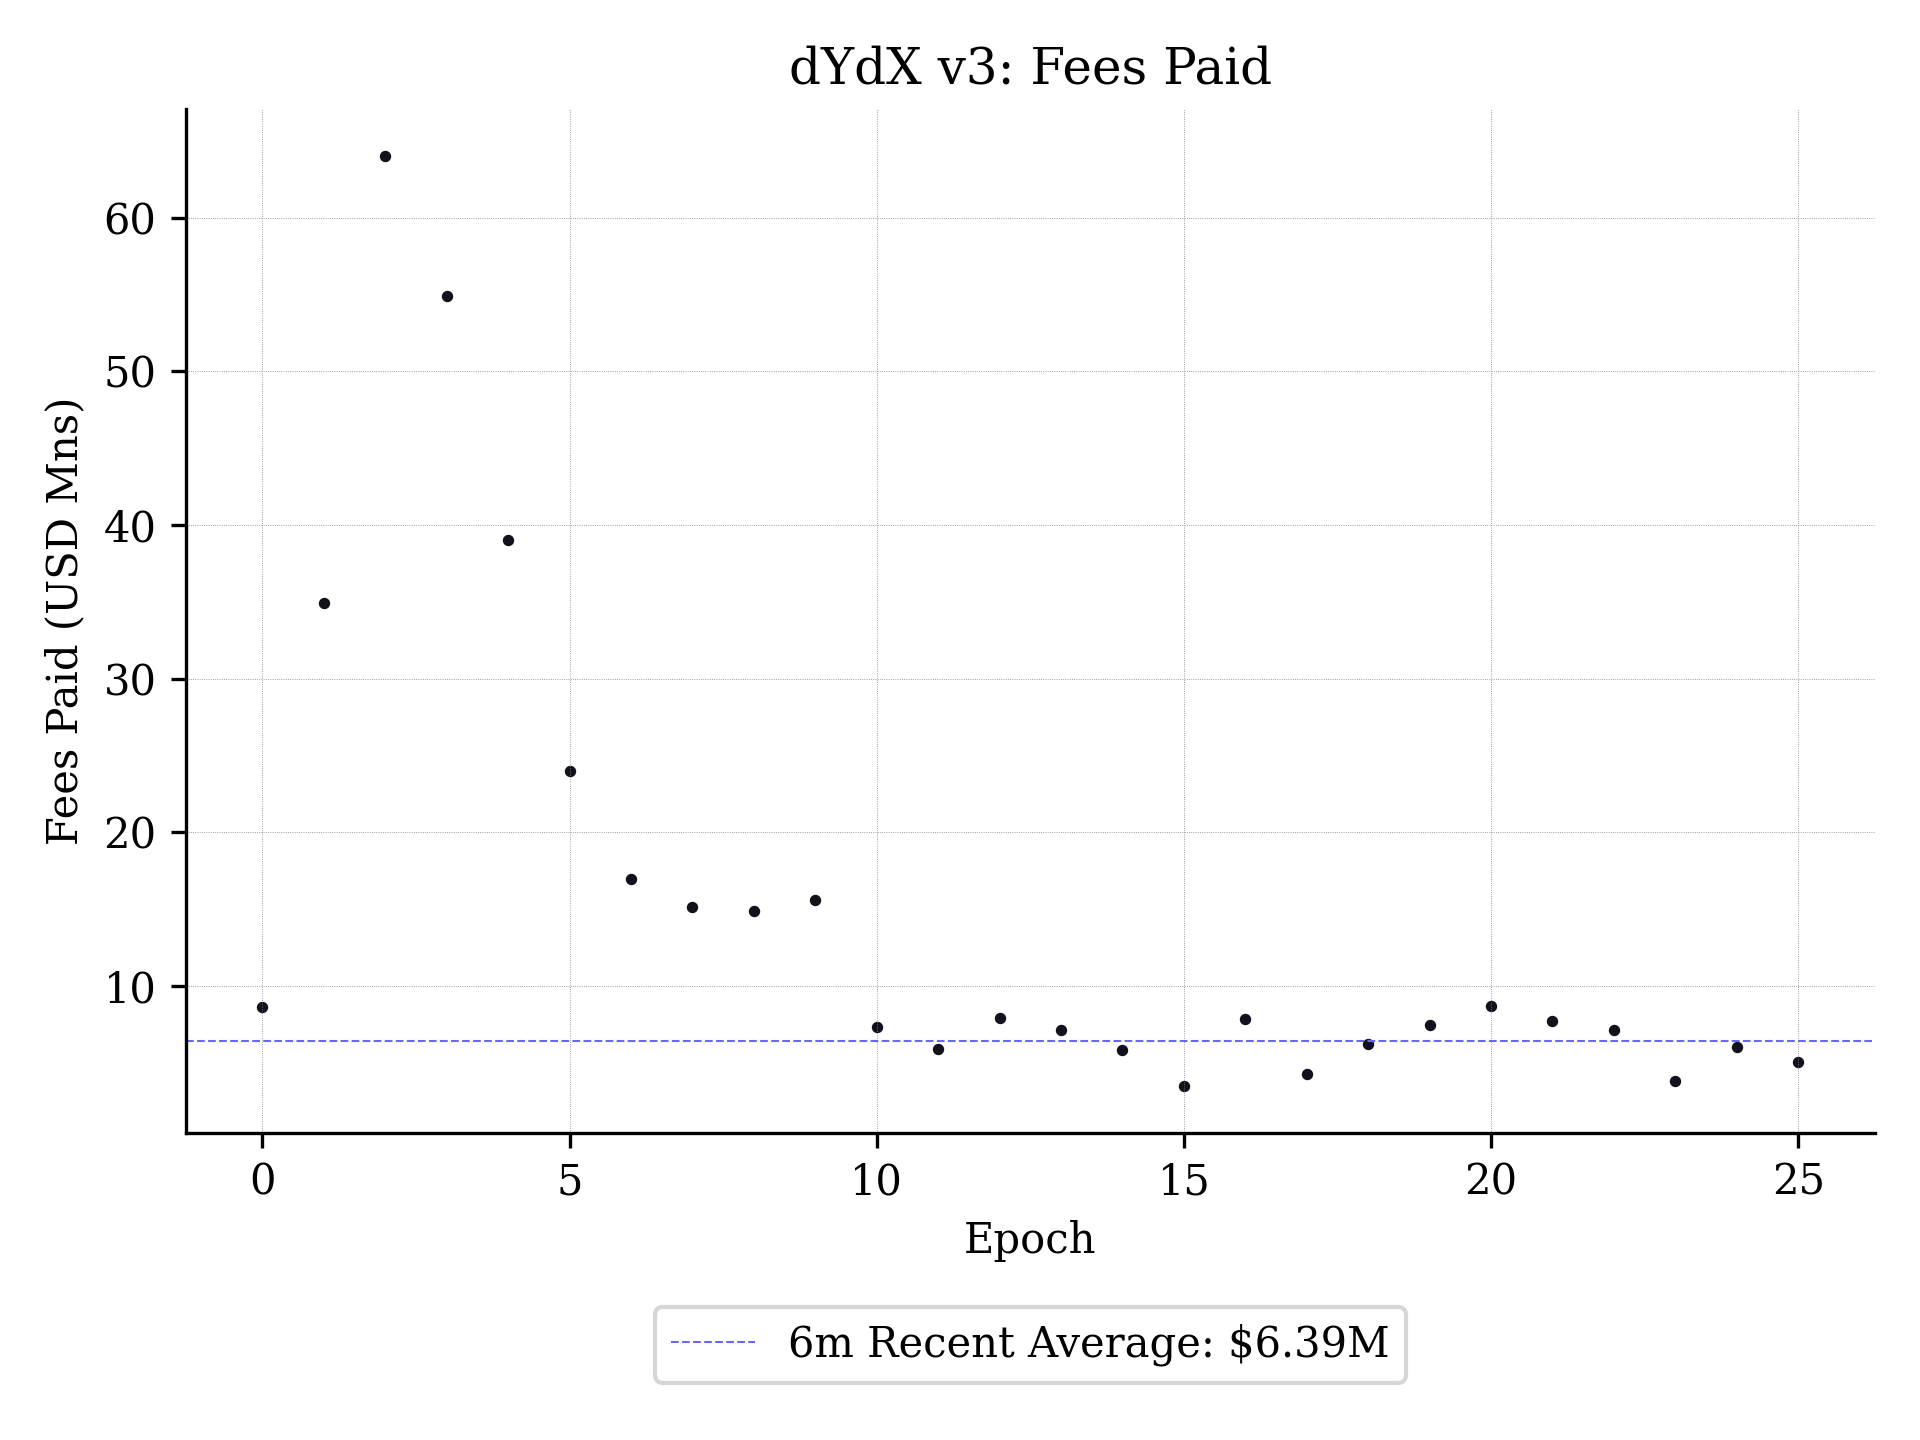
\includegraphics[width=0.6\linewidth]{figs/fees.png}
            \captionsetup{width=.6\linewidth}
            \caption{Fees paid by epoch in dYdX v3. The dotted line indicates the average fees paid between February and July of 2023.}
            \label{fig:fees}
        \end{figure}

        We would like to formulate an incentives program where front end operators are remunerated in proportion to the value they create, which we can measure as a function of their volume generated. In sizing this program, we might first estimate how much trading volume these front ends could realistically generate, and therefore, how much the dYdX community should be willing to pay them. 

        \begin{margintable}
            \small % Reduce the font size in the table as space is at a premium
        \caption{Addressable Market}
        \begin{tabular}{L{0.22\linewidth} C{0.22\linewidth} R{0.25\linewidth}}
            \toprule
            \textbf{Fee-share Pct} & \textbf{DOT Mkt Share} & \textbf{Annual Addressable Mkt}\\
            \midrule
            1\% & 90\% & \$35K \\
            5\% & 90\% & \$177K \\
            10\% & 90\% & \$353K \\
            1\% & 50\% & \$177K \\
            5\% & 50\% & \$883K \\
            10\% & 50\% & \$1,765K \\
            \bottomrule
        \end{tabular}
            \label{table:addressable_mkt}
        \end{margintable}
        
        The gross amount paid in fees to the protocol is displayed in Fig. \ref{fig:fees}. From February to July of 2023, an average $\$6.79M$ USD has been paid in fees on dYdX v3 per epoch. Roughly $40\%$ of trading fees paid to the protocol, meaning that approximately $\$2.7M$ USD is paid in fees through front ends, per epoch. 

        \begin{figure}[htp]
            \centering
            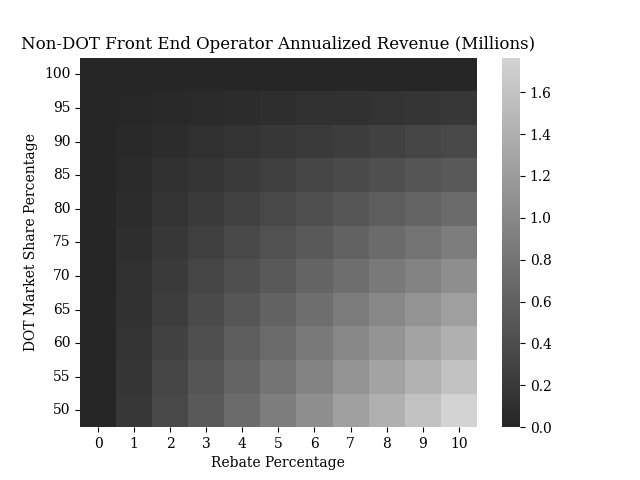
\includegraphics[width=0.7\linewidth]{figs/fee_heatmap2.png}
            \captionsetup{width=.7\linewidth}
            \caption{Fee revenue going to non-DOT operators as a function of the DOT's market share, and fee-share percentage. Assuming total fee revenue of $\$6.79M$, with $40\%$ originating from front ends.}
            \label{fig:fees_heatmap}
        \end{figure}

        Given the dYdX Operations Trust (DOT) will be supporting a front end, funded by the community treasury, it will likely take a large percentage of the front end market share. This significantly reduces the incentive for new teams to deploy, maintain, and innovate on dYdX's front end, if we rely exclusively on a revenue share system. Using recent per-epoch fees, we illustrate the potential size of a fee revenue share program in Fig. \ref{fig:fees_heatmap}, with some example numbers in Table \ref{table:addressable_mkt}. Notice that, even if the DOT is removed from the incentives program entirely, it is likely that the distribution of rewards will still be ``power-lawed''. 

        \nonumsidenote{The DOT was awarded $\$360k$ USD to deploy and maintain all three front ends for dYdX v4.}We denote the percentage of front end fees being shared with front end operators as the \textit{fee-share percentage}. Given that trading fees sustain the app chain's validators, and therefore are fundamental to the security assumptions for dYdX v4, the fee-share percentage must be kept relatively small. In Fig. \ref{fig:fees_heatmap}, we consider some reasonable fee-share percentages, and assume that the DOT controls at least $50\%$ of the front end market. For example, assuming the DOT takes $50\%$ market share and the fee-share percentage is $1\%$, all other front end operators would split an annual $\$177K$ USD, a paltry incentive to decentralize the dYdX front end.

    \subsection{Scoring Rules}

        So far we have assumed that incentives are disbursed \textit{pro-rata} amongst front end operators. We may instead consider two alternative scoring rules for distributing incentives: a logarithmic scoring rule, defined in Eq. \ref{eq:logscore}, and a square-root scoring rule, defined in Eq. \ref{eq:sqrtscore}. As shown in Fig. \ref{fig:simmed_scores}, both scoring rules flatten the distribution of rewards, increasing the incentives for new and smaller teams to participate in the incentives program and deploy new front ends.

        Define the logarithmic scoring rule as

        \begin{equation} \label{eq:logscore}
            R_{i, \log} = \frac{\log{(w_i + 1)}}{\sum_j^N{\log(w_j + 1)}}, 
        \end{equation}

        where there are $N$ participating front ends, $w_i$ is the amount of trading fees routed through the $i$th front end, and $R_{i, \log}$ is their fraction of incentives (fees). Similarly, we define the square root scoring function as

        \begin{equation} \label{eq:sqrtscore}
            R_{i, \sqrt{}} = \frac{\sqrt{w_i}}{\sum_j^N{\sqrt{w_j}}}, 
        \end{equation}

        % \begin{figure}[htp]
        %     \centering
        %     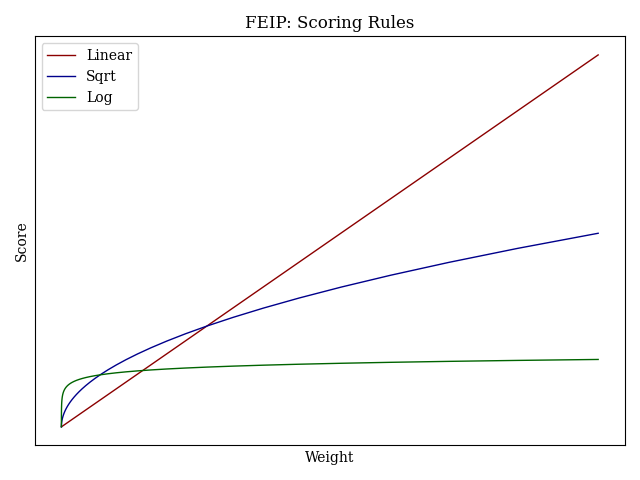
\includegraphics[width=0.7\linewidth]{figs/feip_scoring.png}
        %     \caption{Different scoring rules for the Front End Incentives Program.}
        %     \label{fig:feip_scoring}
        % \end{figure}

        \begin{figure}[H]
            \centering
            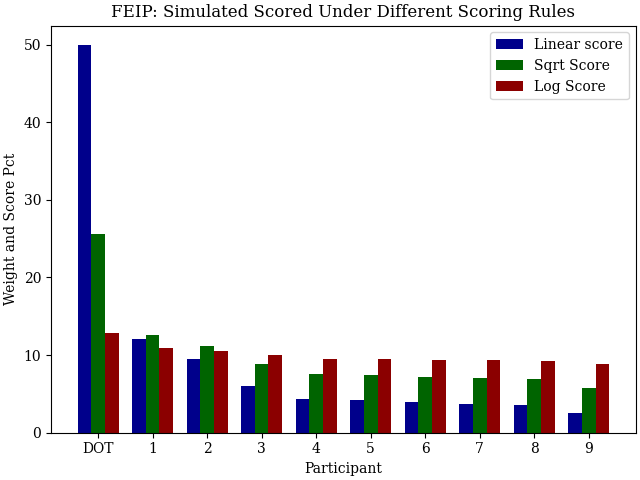
\includegraphics[width=0.7\linewidth]{figs/simmed_scores.png}
            \caption{Simulated scores for the front end incentives under different scoring regimes, assuming the DOT takes $50\%$ market share.}
            \label{fig:simmed_scores}
        \end{figure}

        From Fig. \ref{fig:simmed_scores} it is clear that either scoring rule produces a flatter rewards distribution than a naive \textit{pro-rata} distribution. This significantly increases the incentives for smaller teams to deploy new front ends, and decreases the risk they are unable to service their costs if their front end does not get enough traction. However, the logarithmic scoring rule produces an almost entirely flat curve, largely removing any meritocracy in the incentives program. This is not desirable either: some degree of meritocracy encourages participants to continuously innovate on their product and acquire more customers.

        We may choose to further parameterize our scoring rules to achieve some optimal degree of ``flattness'' in the rewards distribution. For example, we may use a cubed root instead of a square root to further flatten the distribution under a root scoring rule, or we may scale the argument of the log by a constant $k$. Either parameterization could be used to control this flattening process, but introduces complexity in designing the incentives program. To keep the incentives program simple, and remove any operational overhead in designing and maintaining the program, we consider moving forward with the square-root scoring rule. We revise the addressable market size from Table \ref{table:addressable_mkt} in Table \ref{table:addressable_mkt_sqrt} using our newly proposed scoring function. Notice how the incentives, particularly when the DOT takes most of the market share, are significantly higher under a square root scoring function than under the \textit{pro-rata} distribution, by on the order of 5x.

        % \begin{figure}[htp]
        %     \centering
        %     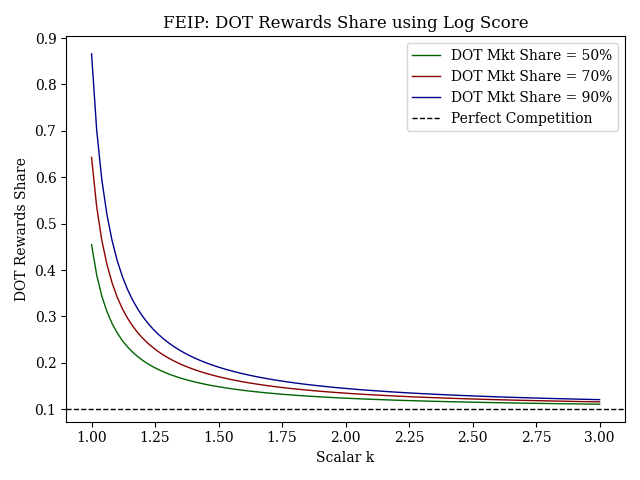
\includegraphics[width=0.7\linewidth]{figs/feip_dot_rewards.png}
        %     \caption{Different scoring rules for the Front End Incentives Program.}
        %     \label{fig:feip_scoring}
        % \end{figure}

        \begin{margintable}
            \small % Reduce the font size in the table as space is at a premium
        \caption{Addressable Market, Sqrt Scoring Rule}
        \begin{tabular}{L{0.22\linewidth} C{0.22\linewidth} R{0.25\linewidth}}
            \toprule
            \textbf{Fee-share Pct} & \textbf{DOT Mkt Share} & \textbf{Annual Addressable Mkt}\\
            \midrule
            1\% & 90\% & \$167k \\
            5\% & 90\% & \$837k \\
            10\% & 90\% & \$1,669k \\
            1\% & 50\% & \$258k \\
            5\% & 50\% & \$1,287k \\
            10\% & 50\% & \$2,573k \\
            \bottomrule
        \end{tabular}
            \label{table:addressable_mkt_sqrt}
        \end{margintable}

        Any non-linear scoring rule would require the incentives to be pooled for some period of time while scores are calculated and then disbursed to participants. A possible implementation of this is to re-use the design of dYdX v3's rewards programs, which rewarded participants in ethDYDX at the end of each epoch. This might entail pooling the rewards for a certain period of time, perhaps a block, perhaps an epoch. The protocol would then track the percentage of trading fees originating from each front end, compute their score, and distribute the proceeds at the end of the measurement period.

        Notice that, under a non-linear scoring rule, front end operators are incentivized to Sybil-attack the incentives program. Instead of building one front end and acquiring users to trade through this front end, operators would be encouraged to create many front ends, and leverage the non-linearity of the scoring rule to get more rewards, without having to contribute more in trading fees to the protocol.
        \sidenotequote{dYdX Trading identified 80 Ethereum addresses (listed below) that conducted clear wash trading during Epoch 0 and removed them from receiving Trading Rewards for Epoch 0.}{\bhref{https://forums.dydx.community/discussion/1677-wash-trading-epoch-0}{Wash Trading - Epoch 0}}
        Furthermore, consider programmatic traders who trade via API instead of front ends, such as market makers or arbitrageurs, that push significant volume on dYdX chain. Under any front end incentives program that does not require a whitelisting process and rewards front ends proportional to their trading activity, these programmatic traders are incentivized to spoof a front end connection to be eligible for rewards. The whitelisting process described in a previous Section eliminates these concerns.
        
    \subsection{DYDX Rewards or Fee Sharing?}

        Although governance will be able to control ``fee-sharing'' on dYdX Chain (for example, using the Community Tax discussed in Section \ref{sec:validators}), there are several reasons the community might want to avoid enabling this feature shortly after the Genesis of dYdX Chain, particularly in ensuring the security of the chain's consensus mechanism. Instead, we consider using DYDX rewards to fund this incentives program, until governance is comfortable enabling a fee share across the dYdX ecosystem. \sidenotequote{Decentralized ecosystems, if properly structured, can use tokens to incentivize participants to contribute value to the ecosystem and correspondingly distribute that value more equitably among system stakeholders according to their contributions. To achieve this, web3 systems need to vest meaningful power, control, and ownership with system stakeholders (via airdrops, other token distributions, decentralized governance, etc.). As a consequence, the value of the ecosystem as a whole accrues to a broader array of participants rather than one central entity and its shareholders. \newline The ongoing balancing of incentives among the stakeholders-developers, contributors, and consumers-can then drive further contributions of value to the overall system, to the benefit of all.}{\bhref{https://a16zcrypto.com/posts/article/decentralization-factors-web3-protocols-tables/}{\textit{Factors of decentralization of web3 protocols}} by Miles Jennings, Stephen Wink, Adam Zuckerman}
        
        If governance were to choose to implement this program using DYDX rewards, we may use the discussions from the previous sections to size this program. First, we would have to modify our square-root scoring rule such that governance does not ``overspend'' on these incentives. We take inspiration from the \bhref{https://dydx.exchange/blog/v4-rewards-and-parameters}{v4 Trader Rewards formula}, discussed in Section \ref{sec:incentives}, which prevents traders from earning more in rewards than they pay in fees. We might similarly set:

        \begin{equation}
            A = \min{\left(\frac{C \cdot S}{p}, T \right)}
        \end{equation}

        where $A$ is the amount in rewards that will be disbursed, $T$ is the maximum amount in rewards that governance is willing to pay, $C$ is the maximum percentage of trading fees that governance is willing to pay, $S$ is the sum of trading fees routed from participating front ends, and $p$ is the price of DYDX. Intuitively, this formula ensures that governance will never overpay for front end incentives: it will always pay at most $C\%$ of the fees routed from that front end. As this functionality will already have been developed by dYdX Trading, it signfiicantly streamlines the implementation of this program. The rewards, $A$, may then be disbursed according to the square-root scoring rule introduced in Eq. \ref{eq:sqrtscore}. 

    \subsection{Summary} \label{subsec:summary_feip}

        dYdX v4 is fundamentally about decentralizing the various components of the protocol, from the orderbook to the front end. In this Section, we have outlined how and why the DAO might implement a whitelisting and curation process for a Front Ends Registry. This Registry signals to retail users which front ends abide by certain community-owned standards and are unlikely to commit any frauds. We then discuss how and why an incentives program might be appropriate to accelerate the decentralization of the dYdX front end, and perhaps contribute to the innovation and improvement of the user experience. We observed that the addressable market for incentivizing front end operators using a fee share is small, particularly given the large market share the dYdX Operations Trust will likely take. We proposed a square root scoring rule for incentivizing small front end operators to maintain new front ends, encouraging the development of front ends in different regions, languages, and perhaps with different functionalities. Finally, we discussed how and why this program might be funded with DYDX rewards instead of a direct trading fee share.